% !TEX root = ../main.tex

\section{Background}
\label{section:background}

In this section, we use a traditional statistical framework as a guideline for multilabel methods~\citep{tukey} \gab{needs a bit more explanation}. We distinguish the desired theoretical statistic (the estimand), its functional form (the estimator) and its approximation (the estimate). We show how multilabel reductions tend to reformulate the estimand and treat labels independently (i.e. change the assumptions about the data). However, with an appropriate estimator, it is possible to directly model the estimand. Our proposed loss function, multilabel blend, accommodates for the true estimand.

For the reminder of the text, we define a learning algorithm that maps inputs to outputs given a set of hyperparameters \(\mathcal{F}(\cdot ; \Theta): \mathcal{X} \rightarrow \mathcal{Y}\). 

\subsection{Estimand: definition of the risk}
\label{section:background:estimand}

Take a classification setting with $C$ classes. Two scenarios are described in the literature, the multilabel and the mutliclass scenario. In the former, a single example can be attributed more than one label of each class (e.g. movie genres). In the latter, a single example has per definition only one label stemming from a class (e.g. classification of an animal on a picture). The multilabel risk can be written as in ~\citep{multilabelReduction}:

\begin{equation}
R_{\mathrm{ML}}(\mathcal{F}) = \mathbb{E}_{(x, y)}\left[\ell_{\mathrm{ML}}(y, \mathcal{F}(x))\right]
\end{equation}

We use the risk as the estimand: the theoretical statistic. \gab{elaborate}

\subsection{Estimator: the functional form of the risk}
\label{section:background:estimator}

The estimator $f \in \mathcal{F}$ is any minimizer of the risk $R_{ML}$. 
Menon et. al. ~\citep{multilabelReduction} define the multiclass setting as any setting that 

\begin{proposition}
the multilabel estimator of $y_i$ shall be dependent on the input and other labels,
\begin{equation}
  \hat{y}_i = \mathcal{F}(x, y_1, ..., y_C) = P(y_i | x, y_1, ..., y_C) \forall y_j not in y_i
\end{equation}
\end{proposition}

Predicting multiple labels per example comes with the assumption that labels are non-mutually exclusive. By proposing this general formulation, we entrench that characteristic in the estimator.

Contrary to Menon et. al. ~\citep{multilabelReduction}, we propose an estimator that models interdependence between labels and deals with thresholding for the estimate for free (see next section).

Multilabel reduction methods are characterized by their way of reformulating the estimand, the resulting estimator and the estimate. In particular, this allows the use of existing losses: logistic loss, sigmoid loss or softmax cross-entropy loss.


\subsection{Estimate: approximation via a loss function}
\label{section:background:estimate}

Given the general non-convex optimization context, the loss function $\ell(y_i, hat{y_i})$ can take different forms. 

\textbf{One-versus-all}

\begin{equation}
\ell_{\mathrm{OVA}}(y, f) \doteq \sum_{i \in[L]} \ell_{\mathrm{BC}}\left(y_{i}, f_{i}\right)=\sum_{i \in[L]}\left\{y_{i} \cdot \ell_{\mathrm{BC}}\left(1, f_{i}\right)+\left(1-y_{i}\right) \cdot \ell_{\mathrm{BC}}\left(0, f_{i}\right)\right\}
\end{equation}

with $\ell_{\mathrm{BC}}$ some binary classification loss, most often logistic loss.  Note that minimizing binary cross-entropy is equivalent to maximizing for log-likelihood
\cite[Section 4.3.4]{Bishop}. Cross-entropy loss can be formulated as \(\mathcal{L}_{\text {CE}}=-\sum \log \left(p_{i}\right)\).

\textbf{Pick-all-labels}

\begin{equation}
\ell_{\mathrm{PAL}}(y, f) \doteq \sum_{i \in[L]} y_{i} \cdot \ell_{\mathrm{MC}}(i, f)
\end{equation}

\textbf{Pick-one-label}

For this reduction, given an example $(x,y)$, a single random positive label is chosen as the true label of $x$


Note that OVA and PAL have each a form normalised by the number of positive labels, 


Conveniently, these multilabel reductions allow the use of known losses such as logistic loss (for binary classification formulations), sigmoid loss or softmax crosss-entropy loss (for multiclass formulations). Note that all these reductions imply a reformulation of the estimator as follows:

\begin{equation}
  y_i = \mathcal{F}(x) = P(y_i | x)
\end{equation}

This time, we assume independence of labels propensities. \gab{the reformulation of the estimator also implies a reformulation of the estimand like so...}


Note that multilabel reductions was earlier sometimes referred to as \emph{fit-data-to-algorithm} solutions (a.k.a. \emph{problem tranformation}) as opposed to \emph{fit-algorithm-to-data} solutions (a.k.a.\ \emph{algorithm adaptation})~\cite{multilabelReview, multilabelReview2}. In Section~\ref{section:background:fitdata} we propose a fit-algorithm-to-data solution (i.e. a loss function), where the estimand and assumptions about the data are not reformulated.

Note the special case of hierarchical labeling. With a hierarchical structure in labels, one can constrain the algorithm to learn only 1 or $k$ labels per group in the hierarchy. For example, DBPedia~\citep{lehmann2015dbpedia} establishes a hierarchical structure in Wikipedia infoboxes and is commonly used to finetune state-of-the-art NLP models~\citep[see, e.g.,][]{XLNet, ULMFit}. Hierarchical labeling thus comes with different predicates than other multilabel classification problems and are out of scope.

Note that for many real world problems and datasets reducing the problem to top-k selection or establishing a hierarchical structure is an oversimplification, especially when classes are not mutually exclusive. Besides the four datasets we use for our experiments, we mention others in the related work section.

\subsection{Metrics: evaluation at inference time}
\label{section:background:metrics}

There is a consensus around the use of confusion matrix metrics (CMM) to evaluate multilabel classification models (at inference time). Notably Precision and Recall. CMMs come with caveats: most of these measures (I) require a hard thresholding, (II) they are very sensitive to the choice of the number top labels to include $k$~\footnote{In the case of unilabel prediction, top-k becomes a top-1 problem, which essentially eliminates caveats I and II.} and (III) they require choices to be made in terms of  micro / macro / weighted metrics.

Some common CMMs are Precision, Recall, F1-score, hinge-loss or one-error-loss. Numerous others can be found on the confusion matrix Wikipedia page.


We propose a generic loss which does not require hard thresholding decisions, , 


\textbf{consistency}

Similarly to Menon et. al. ~\citep{multilabelReduction} and in the lineage of ~\citep{consistency-surrogates, consistency-multiclassSVM, consistency-lossAnalysis}, we can define consistency as

\begin{equation}
\operatorname{reg}\left(f_{n} ; \ell_{\mathrm{ML}}\right) \rightarrow 0 \Longrightarrow \operatorname{reg}\left(f_{n} ; \ell_{\mathrm{top}-k}\right) \rightarrow 0
\end{equation}

with $reg(f)$ the regret of an estimator with respect to its loss $l_{MC}$ is $\operatorname{reg}\left(f ; \ell_{\mathrm{ML}}\right) \doteq R_{\mathrm{ML}}(f)-\inf _{g: x \rightarrow \mathbb{R}^{L}} R_{\mathrm{ML}}(g)$

a metric is defined as consistent if \gab{elaborate}


\subsection{Multilabel blend estimate: F1 Metric as a Loss}
\label{section:background:metricsAsLosses}

This is our contribution. Similar to lambdaLoss and others... It implicitly deals with label counts and label predictions. It is also consistent and balances precision and recall \gab{elaborate in words and math}


In a number of retrieval tasks, a model's out of sample accuracy is measured
on metrics such as AUROC, F1 score, etc. These reflect an objective catered
towards evaluating the model over an entire ranking. Due to the lack of
differentiability, these metrics cannot be directly used as loss functions at
training time (in-sample). A seminal study~\cite{optimizableLosses} derived a
general framework for deriving decomposable surrogates to some of these
metrics. We propose our own decomposable surrogates tailored for the problem
at hand.

In a typical machine learning classification tasks, binary labels are compared to a probabilistic measure (or a reversible
transformation of a probabilistic measure such as a sigmoid or a softmax
function). If the number $n_i$ of labels to be predicted per
example is known a priori, it is natural at training time to assign the $top_{n_i}$ predictions
to that example~\cite{lossTopKError, topKmulticlassSVM}. If the number of
labels per example is not known a priori, the question remains at both training and at inference time
as to how to decide on the number of labels to assign to each
example. This is generally done via a \emph{decision threshold}, that can be set globally for all
examples. This threshold can optimize for specificity or
sensitivity~\cite{decisionThreshold}. We propose an approach where this threshold
is implicitly defined, by using a loss function that penalizes explicitly for wrong label counts.



\subsection{Multiclass classification}
\label{section:background:multiclassClassification}

Multiclass classification, can be seen as a subdomain of multilabel classification~\citep{multilabelReduction}, where Y = {0, 1}, is arguably more straightforward. Existing loss functions, such as sigmoid loss or softmax cross-entropy loss are already suited to the purpose \gab{explain why}. Note that certain loss functions such as the focal loss accommodate for cases with unbalanced class distributions. 

The multiclass risk can be defined as:

\begin{equation}
R_{\mathrm{MC}}(\mathcal{F}) = \mathbb{E}_{(x, z)}\left[\ell_{\mathrm{MC}}(z, \mathcal{F}(x))\right]
\end{equation}

As we work our way down to the estimator and the estimate, it is clear that existing loss functions are able to deal with the problem at hand without any need of reformulations. \gab{elaborate}



% \begin{figure}[t]
% \centering
% 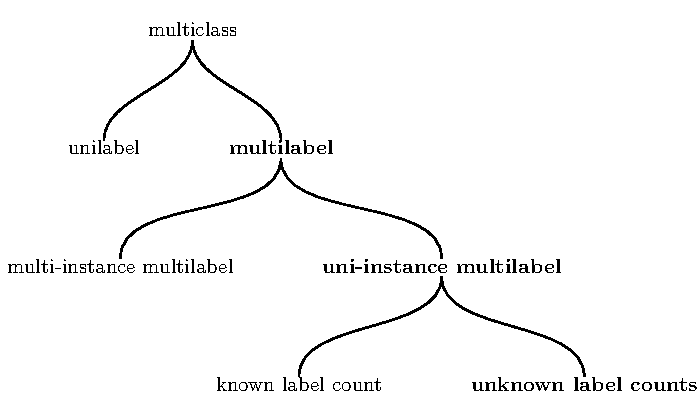
\includegraphics[width=.9\linewidth]{./tree/Tree.pdf}
% \caption{\label{fig:tree} SIMPUL (bold) within the \emph{multiclass}
% nomenclature
% \hvk{figure is not referenced in text, bold is unclear in figure}
% \daan{I think it should go. And if it stays: uni -> single.}
% % Clarifying ``multiclass'' classification problems. In this paper we focus on
% % the uni-instance, multilabel, multiclass classification problem with a
% % varying number of labels (the bottom right hand side of the tree).
% }
% \end{figure}% \mdr{Image source ...}

%%% Local Variables:
%%% mode: latex
%%% TeX-master: "../main"
%%% End: